%!TEX root = ../Thesis.tex

% 1.3 Outline
% The outline gives an overview of the main points of your thesis. It clarifies the structure of your thesis and helps you find the correct focus for your work. The outline can also be used in supervision sessions, especially in the beginning. You might find that you need to restructure your thesis. Working on your outline can then be a good way of making sense of the necessary changes. A good outline shows how the different parts relate to each other and is a useful guide for the reader.

\section{Outline}
This thesis consist of \ref{total:chapters} chapters. It starts with the general introduction you are reading now, which outlines the topic of the work being done.
%, hopefully giving pleasant to read opening. 

In the next chapter, knowing current state of art and being aware of the limitations I have written theoretical considerations. They are base for the implementation part as well as a reference point for analysing and discussion.

It has been followed by a description of the design process in chapter 3. Which naturally evolves into methods being implemented in final stadium described in chapter 4. In this chapter, I have placed a comprehensive description of my design choices, used setup and implementation itself. This part is directly followed by information of how I did test my system and how well it performs against my theoretical considerations.

Then I let myself describe directions for the future implementation which I hope will come in handy for future teams taking care of this project.

A whole text is closed with a few closing comments from me, retrospection on the whole process of building an electric racing car and my part in it.

\todo{Delete rest?}
Beside the mentioned hierarchy, it has been formed to follow two additional nested level. In each chapter, the following sections are sorted in the way to reflect the propagation of CAN messages in the system.

\begin{figure*}[h]
    \centering
            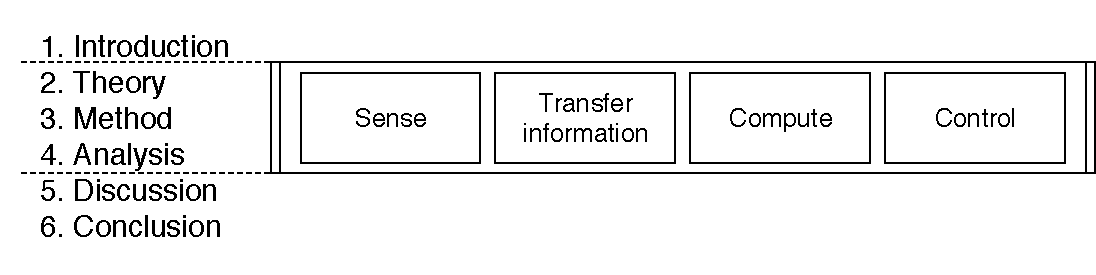
\includegraphics[width=0.8\textwidth]{figures/Outline}
            \label{outline}
            % \caption{CAN and CANOpen timing overview}
\end{figure*}